\chapter{The Solution}

\section{Analytical Work}
\label{sec:prob}
To calculate the probability of a bet occurring, the following calculations are used.

Note that $l \in \{2, 3, 4, 5, 6\}$ and that anywhere that mentions ``occurrences of the value $l$'' should read as occurrences of the value $l$ (or {\Large\epsdice{1}}).
\begin{itemize}
    \item Since {\Large\epsdice{1}}'s are wild, this means that the probability of landing on any die face except 1 is \sfrac{1}{3}.
    \item Let $a_{n, k, l}$ be the event that among $n$ dice, there are exactly $k$ occurrences of the value $l$. Calculating the probability of $a_{n, k, l}$ amounts to rolling $k$ times the value $l$ and $ n - k$ times one of the other faces. By taking the first $k$ positions we get $2^k \times 4^{n-k}$. Now multiplying this result by the set of possible combinations of $k$ positions among $n$ dice, gives
    \[
        \binom{n}{k}2^k4^{n - k}
    \]
    We also have that $\text{Card}(\{1,2,3,4,5,6\}) = 6^n$. From this we get that
    \begin{equation}
        \label{eq:prob_a}
        P(a_{n,k,l}) = \binom{n}{k}\frac{2^k4^{n-k}}{6^n} = \binom{n}{k}\frac{2^k2^{n-k}2^{n-k}}{6^n} = \binom{n}{k}\frac{2^n2^{n-k}}{6^n} = \binom{n}{k}\frac{2^{n-k}}{3^n}
    \end{equation}

    \item Now let $A_{n, k, l}$ be the event that among $n$ dice, there are at least $k$ occurrences of the value $l$. To calculate the probability of $A_{n,k,l}$, we have to sum the probabilities for all $a_{n, i, l}$, $\forall i \in [k, n]$.
    \begin{equation}
        \label{eq:prob_a1}
        P(A_{n,k,l}) = \sum_{i = k}^n\binom{n}{i}\frac{2^{n-i}}{3^n}
    \end{equation}
    \item We can improve upon \Cref{eq:prob_a} by using the player's own dice to factor into the calculation. The event $a_{n, k ,l} \mid a_{m, j, l}$ can be interpreted as the event of having exactly $k$ occurrences of the value $l$ among $n$ dice knowing that we already have $j$ occurrences of the value $l$ among the player's $m$ dice. This is exactly the same as saying, we have exactly $k - j$ occurrences of the value $l$ among $n - m$ dice. Therefore we have
    \[
        a_{n, k ,l} \mid a_{m, j, l} = a_{n - m, k - j, l}
    \]
    and
    \begin{equation}
        \label{eq:prob_b}
        P(a_{n, k ,l} \mid a_{m, j, l}) = \binom{n - m}{k - j}\frac{2^{n-m-k+j}}{3^{n-m}}
    \end{equation}

    \item We can also improve upon \Cref{eq:prob_a1} by using the probability described in \Cref{eq:prob_b}. Let $A_{n, k ,l} \mid a_{m, j, l}$ be interpreted as having at least $k - j$ occurrences of the value $l$ among $n - m$ dice. Then
    \begin{equation}
        \label{eq:prob_b1}
        P(A_{n, k ,l} \mid a_{m, j, l}) = \sum_{i = k - j}^{n - m}\binom{n-m}{i}\frac{2^{n-m-i}}{3^{n - m}}
    \end{equation}
\end{itemize}

The implementation of \Cref{eq:prob_a1} and \Cref{eq:prob_b1} can be seen in \Cref{code:impa1} and \Cref{code:impb1}.
\section{Server Design}

The game hosting platform was built using the \docs{socket} library that comes installed with Python using the terminal as the user interface.

\subsection{Things to note}

\begin{itemize}
    \item The \docs{pickle} package is used to encode and decode data. This package implements binary protocols for serializing and de-serializing a Python object structure.\autocite{pickle}. This allows data that was encoded with \texttt{pickle} to be decoded to it's original type instead of converting the data to a string, converting that string to bytes, sending it to the player, the player converting the bytes back to a string and then to whatever type it should be. This means that the player does not need to have any idea what type the data read in should be converted to. Another advantage of using this package is that allows the server to work in both \texttt{Python2} and \texttt{Python3} as the \texttt{bytes} object that \texttt{Python3} provides does not work in \texttt{Python2}.
    \item Each player is a tuple \texttt{(conn, address)} where conn is a new socket object usable to send and receive data on the connection, and address is the address bound to the socket on the other end of the connection. So calling \texttt{player[0]}(\ref{code:p1}) allows the server to access the socket object to send information to the player.
    \item The \texttt{socket.recv()} method waits until in receives data to proceed to the next line of code.
\end{itemize}

\begin{myminted}{Sending Player information}{p1}
    player[0].sendall(pickle.dumps(self.total_dice))
    player[0].recv(131072)
    player[0].sendall(pickle.dumps(self.player_list[player].dice_list))
    player[0].recv(131072)
\end{myminted}

\subsection{Server Communication}

Using \Cref{im:inround}, the order of operations of the server will be described.

\begin{enumerate}
    \item The server sends each player the number of games they will be playing. Before sending the information to the next player, it waits until the previous player sends an ``OK'' response before continuing.
    \item Each player is sent whether the player is out and if the game is over. Similar to above the server waits until it receives a response before proceeding.
    \item If a player is not out then they are sent their dice.
    \item A player is asked to place a bet.
    \item The bet placed is then sent to all the other players.
    \item Steps 2-5 are repeated until there is only one player left with dice.
    \item After the game is finished, each player is sent a message stating if they have won or lost.
\end{enumerate}

\begin{figure}
    \centering
    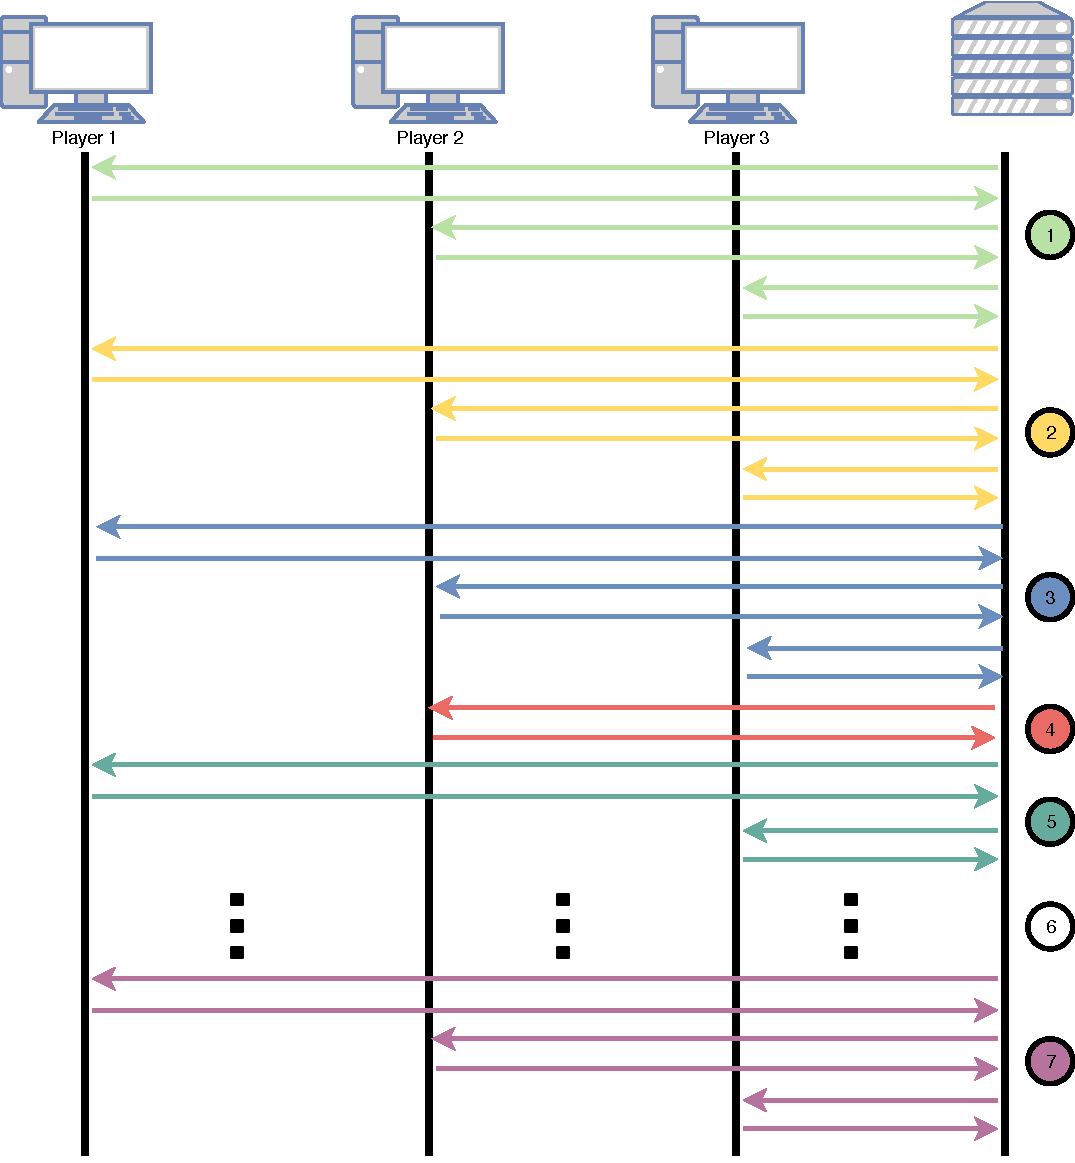
\includegraphics[width=\textwidth]{server.pdf}
    \caption{Order of operation during a game}
    \label{im:inround}
\end{figure}

\section{Methods}
\label{sec:methods}
\subsection{Generating Bets}

The amount of dice to bet on were generated randomly using a skewed normal distribution using the \hackage{scipy} package and the die value to bet on was generated using previous bets. The implementation can be seen in \Cref{code:genbets}.

\noindent The skewed PDF implementation in \texttt{scipy} is generated using

\begin{align*}
    PDF_{\text{Skew}}(x, a, l, s) &= \frac{2 * PDF(y) * CDF(a * y)}{s} \\
    y &= \frac{x - l}{s}
\end{align*}

where $a$ is a skewness parameter, $l$ is a location parameter, $s$ is a scaling parameter and $PDF$ and $CDF$ are the probability density function and cumulative density function, respectively, of the normal distribution. The graph seen in \Cref{im:skewnorm} was generated with $a = 5, l = .5, s = 4$.

\begin{figure}
\centering
\subfloat[PDF of a Skewed Normal Distribution]{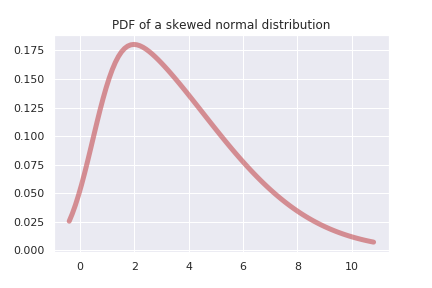
\includegraphics[width=.45\textwidth]{skewnorm.png}\label{im:skewnorm}}
\hfill
\subfloat[Probability of a bet with 10 dice in play]{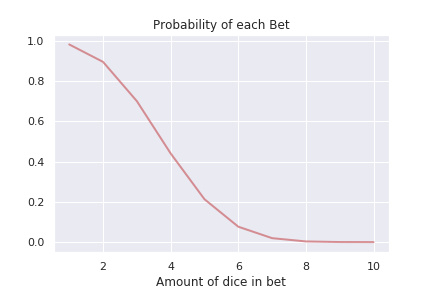
\includegraphics[width=.45\textwidth]{diceprob.png}\label{im:diceprob}}
\caption{Skewnorm compared to dice probability}
\end{figure}

A skewed distribution was used as, when placing bets, it is usually safer to place a low number of a die value. If a standard normal distribution was used instead of a skewed distribution, every amount would be just a likely when generating bets. However in the game this is not the case as bets that contain a high dice number a less likely to occur as seen in \Cref{im:diceprob}, where the $x$-axis is the amount of dice that you are betting are on the table.\\

The die value itself was generated using bets made throughout the round. The code is more likely to generate a number that has already been bet on as it is more likely that there are more dice on the table, with a die value that has already been bet on.

\subsection{Improving the Probability Formula}

The formulas seen in \Cref{sec:prob} do not take into account the bets that have been made in the current round. Suppose that $D$ is a dictionary containing the numbers 2 to 6 as the keys and the values being the highest amount of that die value that has been bet. Then
\begin{equation}\label{eq:fkl}
    f(k, l) = P(A_{n, k, l} | a_{m, j, l}) + D[l]
\end{equation}
where $j, k, l, m$ and $n$ are as described in \Cref{eq:prob_b1}. Note that this is no longer a probability but rather a score metric as we can obtain values larger than 1. The implementation can be seen in \Cref{code:fkl}

\subsection{Minimax}

Minimax is a depth-first depth-limited search which examines all states . There are 2 phases in the algorithm
\begin{enumerate}
    \item Descend the search tree up to the depth limit and apply the heuristic function.
    \item Propagate those values up the tree.
\end{enumerate}

The basic idea of Minimax is that during your move you want to maximize the heuristic value, as this is the best move for you, while the opponent tries to minimize the heuristic value as this will result in you performing a worse move.

\subsubsection{Example of Minimax}
\begin{figure}
    \centering
    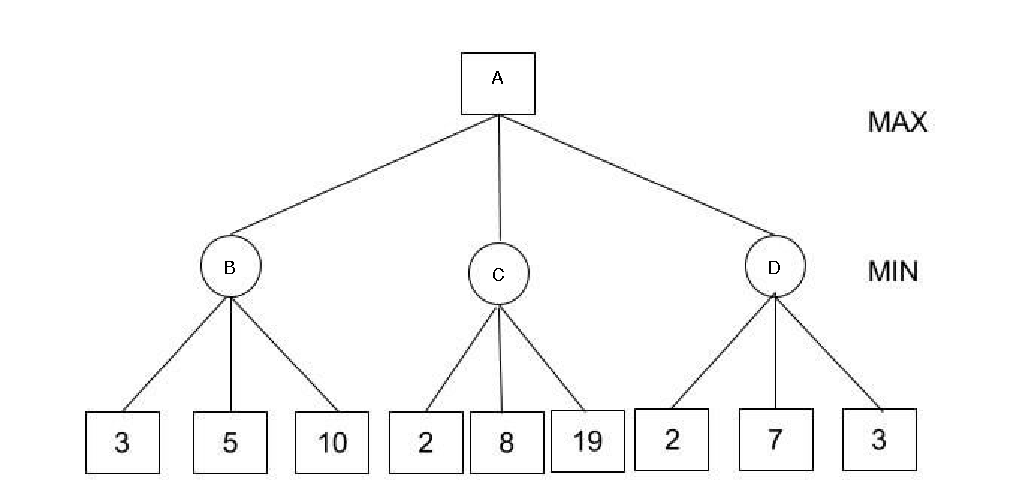
\includegraphics[width=\textwidth]{minimax.pdf}
    \caption{Minimax Tree}
    \label{im:minimax}
\end{figure}

We traverse the tree depth-first, starting from the left branch.

\begin{enumerate}
    \item Since B is a minimizer, it will pick the child node that has the lowest heuristic value. In this case B now has a value of 3.
    \item C is a minimize so it will pick the node that has a heuristic value of 2. Now C has a heuristic value for 2.
    \item D is a minimize, so it picks the child with a heuristic value of 2. D now has a value of 2.
    \item Since A is a maximizer, it picks the child node with the highest heuristic value. In this case that would B.
    \item Therefore we will perform the action that node B represents.
\end{enumerate}

The implementation for this can be seen in \Cref{code:minimaximp}

\subsection{$\alpha$--$\beta$ pruning}

The problem with regular Minimax is that it is an exhaustive method that explores unnecessary search spaces causing the algorithm to be slow and inefficient. For this reason $\alpha$--$\beta$ pruning will be used.

In $\alpha$--$\beta$ pruning there are two threshold values:
\begin{itemize}
    \item $\alpha$, which represents the lower bound of a maximizing level.
    \item $\beta$, which represents the upper bound of the minimizing level.
\end{itemize}

We terminate a search when we are
\begin{itemize}
    \item below a max node with $\alpha \geq \beta$ of any of it's min ancestors.
    \item below a min node with $\alpha \geq \beta$ of any of it's max ancestors.
\end{itemize}

Let $b$ be the number of children for each node and $m$ is the maximum depth of the tree then:
\begin{itemize}
    \item For regular MiniMax, the time complexity is $\mathcal{O}(b^m)$.
    \item For MiniMax with $\alpha$--$\beta$ pruning, the time complexity is $\mathcal{O}(b^{m/2})$
\end{itemize}

With the termination rules above, we can easily modify the implementation seen in \Cref{code:minimaximp} so that it implements $\alpha$--$\beta$ pruning, as seen in \Cref{code:abpruning}

\subsubsection{Example}

We will work through a partial example of how $\alpha$--$\beta$ pruning works by looking at the tree below.

\begin{figure}
    \centering
    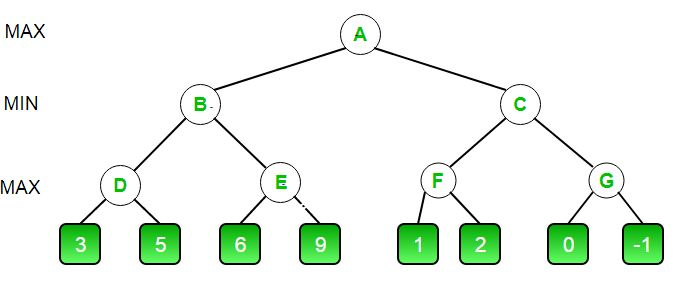
\includegraphics[width=\textwidth]{MIN_MAX1.jpg}
\end{figure}

\begin{enumerate}
    \item The initial call starts from A. Initially, $\alpha = -\infty$ and $\beta=\infty$. These values are passed down to subsequent nodes in the tree. We then explore the left branch of the tree.
    \item At D, it has $\alpha = -\infty$ and $\beta = \infty$ as these are inherited from A.
    \item D looks at it's left child which returns a value of 3. Now $\alpha = \max(-\infty, 3) = 3$.
    \item Since $\alpha = 3 \not\geq \beta$ we continue searches other children of D.
    \item D looks at it's right child which returns a value of 5. Now $\alpha = \max(3, 5) = 5$.
    \item D then returns a value of 5 to $B$. Now B has $\beta = \min(\infty, 5) = 5$.
    \item Now the right child of B is explored. At E, $\alpha = -\infty$ and $\beta = 5$.$\beta \neq \infty$ as B passes it's value down to E.
    \item E looks at it's left child, which returns 6. Now $\alpha = \max(-\infty, 6) = 6$.
    \item Since $\alpha = 6 \geq \beta = 5$, we do not need to check the other child of E. This is because B is a minimizing node and as D guarantees that it will return \underline{at most} 5, while after exploring the left child of E, we know it will return \underline{at least} 6, Therefore exploring along the right child of E is useless as we will never pick E.
\end{enumerate}

After performing the algorithm on the whole tree, we end up with the resulting search space seen in \Cref{im:finaltree}

\begin{figure}
    \centering
    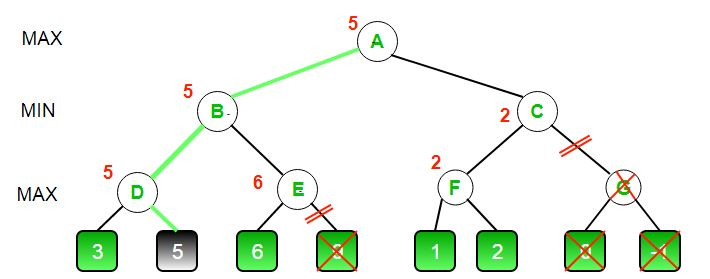
\includegraphics[width=\textwidth]{MIN_MAX3.jpg}
    \caption{Final Tree after performing $\alpha$--$\beta$ pruning}
    \label{im:finaltree}
\end{figure}

In this example we saved time compared to the regular Minimax algorithm by not exploring 3 nodes. In larger graphs the number of nodes that are not explored in the $\alpha$--$\beta$ pruning version of Minimax is a lot larger than this. This means we save time searching and this allows us to search more nodes in the same amount of time.



\section{Class Structure}

\begin{figure}
    \centering
    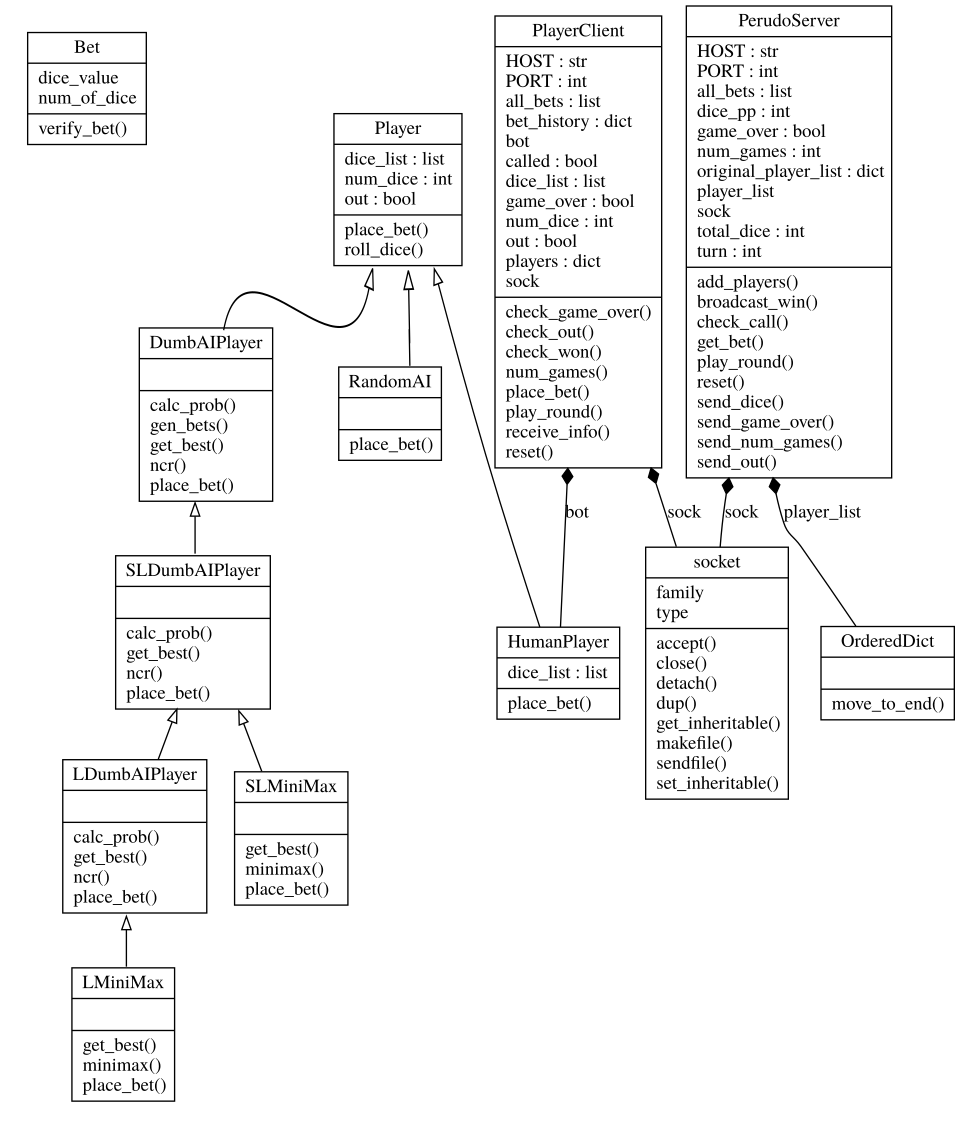
\includegraphics[width=\textwidth]{classes.png}
    \caption{UML Class Diagram of Project}
    \label{fig:class}
\end{figure}

The class structure of the project this project can see seen in \Cref{fig:class} and the dependency graph can be seen in \Cref{fig:package}.

\begin{figure}
    \centering
    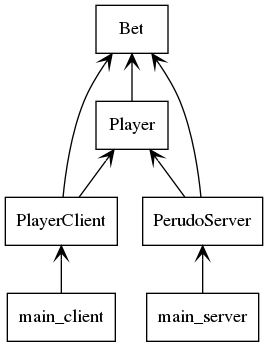
\includegraphics[scale=.5]{packages.png}
    \caption{Package Structure of Project}
    \label{fig:package}
\end{figure}

\section{Implementation}
\subsection{Strategy for AIPlayer's}

The general strategy for all the AI's except MiniMax is as follows
\begin{enumerate}
    \item If you are placing a starting bet then bet that there are at least 2 to 4 dice of some number.
    \item If you are not placing a starting bet, then generate bets using the method seen in \Cref{sec:methods}.
    \item If the probability (or score), calculated using \Cref{eq:prob_a1} for \texttt{DumbAIPlayer} and \Cref{eq:prob_b1} for \texttt{SLDumbAIPlayer} and \Cref{eq:fkl} for \texttt{LDumbAIPlayer}, for any bet is less than the \texttt{prob} value passed into the function then the AI calls the previous players bet and goes back to step 1.
    \item Otherwise, the AI then places a random bet from the generated bets with a probability given by the \texttt{bluff} variable or it places the bet from the generate bets that has the highest probability.
\end{enumerate}
The actual implementation for placing bets can be seen in \Cref{code:getbest}.

\subsection{Strategy for MiniMax}

The strategy that the both \texttt{LMiniMax} and \texttt{SLMiniMax} players is as follows
\begin{enumerate}
    \item If you are placing a starting bet then bet that there are at least 2 to 4 dice of some number.
    \item If you are not placing a starting bet, then run the \texttt{minimax()} method (\Cref{code:abpruning})
    \item If the score, calculated using \Cref{eq:fkl} for \texttt{LMiniMax} and \Cref{eq:prob_b1} for \texttt{SLMiniMax}, for the bet returned by the \texttt{minimax()} method is less than the \texttt{prob} value passed into the function then the AI calls the previous players bet and goes back to step 1.
    \item Otherwise, either the AI places a random bet like above or it places the bet output by the \texttt{minimax()} method.
\end{enumerate}
The implementation can be seen in \Cref{code:mmbet}.
